\documentclass[12pt,a4paper]{ctexart}

\usepackage{geometry}
\usepackage{graphicx}
\usepackage{booktabs}
\usepackage{longtable}
\usepackage{array}
\usepackage{float}
\usepackage{hyperref}
\usepackage{xcolor}
\usepackage{caption}
\usepackage{subcaption}
\usepackage{enumitem}

\geometry{margin=2.3cm}
\hypersetup{colorlinks=true,linkcolor=blue!60!black,urlcolor=blue!60!black}
\captionsetup{font=small}

\title{\textbf{健康数据洞察：全球疾病谱演变、风险归因与卫生资源配置分析}}
\author{HdI 项目组}
\date{2026年3月}

\begin{document}
\maketitle

\begin{abstract}
本研究基于赛题提供的 5 类数据集，对 2000--2023 年全球 203 个国家和地区的疾病谱演变、风险因素归因与卫生资源配置效率开展了数据优先的系统分析，并对中国近 20 年卫生数据进行了省级补充刻画。研究首先将全球死亡原因数据归并为“传染性疾病、非传染性疾病、伤害”三大类，构建国家--年份主面板；随后结合 HNP 与 WDI 指标，分析健康结果差异与资源条件。结果显示：2023 年全球非传染性疾病死亡占比达到 74.57\%，说明全球疾病谱转型已经非常明显；日本的预期寿命最高（约 84.0 岁），乍得最低（约 53.0 岁）；以最新截面估计，预期寿命与人均 GDP 呈显著正相关（$R^2=0.906$）。在风险归因方面，2023 年全球归因死亡规模最大的风险因素为高血压，对应归因死亡约 1083.5 万；AFRO 地区最突出的风险则转向“儿童和孕产妇营养不良”。在资源配置方面，索马里、乍得、尼日利亚等国呈现最明显的“理论需求高于实际配置”的缺口，另有 26 个国家落入“低投入--高产出”象限，显示出值得推广的效率经验。研究最终形成了可复现的数据处理程序、静态 API 输出、图表与 AI 协作记录，为后续在和鲸平台复现与展示提供了完整基础。
\end{abstract}

\section{研究背景与任务理解}
健康中国与 SDG 3 都强调“改善健康结果、降低风险暴露、优化资源配置”必须放在同一分析框架中。与传统只讨论单一疾病或单一指标的做法相比，本赛题更强调用多源数据描述健康生态系统，并在此基础上给出可复现、可解释、可执行的洞察。

本项目围绕赛题的三个核心维度展开：
\begin{enumerate}[label=\arabic*)]
    \item 描述全球疾病谱从传染性疾病向非传染性疾病转移的时空过程，并量化健康指标差异；
    \item 分析主要风险因素对全因死亡的归因贡献，并构建未来情景模拟与优先干预清单；
    \item 评估各国卫生资源投入与健康产出的匹配程度，识别资源不足或低效率区域，并给出再分配见解。
\end{enumerate}

\section{数据来源与处理流程}
\subsection{数据来源}
本研究使用赛题提供的全部 5 类数据：
\begin{itemize}[leftmargin=1.5em]
    \item 全球各国核心疾病与死亡数据：2000--2023 年，22 个死亡原因；
    \item 全球各国健康风险因素数据：2000--2023 年，20 个风险因素；
    \item 全球各国健康营养和人口统计数据（HNP）；
    \item 全球社会经济发展背景数据（WDI）；
    \item 全国近 20 年卫生数据（中国省级与全国汇总表）。
\end{itemize}

\subsection{清洗与标准化}
真实 provided 数据与原始脚手架假设存在明显差异，因此本项目没有继续沿用虚构的 \texttt{daly\_rate}、\texttt{GHRI}、严格暴露率--相对危险度输入，而是做了三项关键重构：
\begin{enumerate}[label=\arabic*)]
    \item 为每类数据建立单独清洗器，先做中文列名映射，再做统一标准化；
    \item 使用 World Bank 国家元数据与 Babel 中文地名表构造国家名到 ISO3 的本地映射，修复中文国家名与 Unicode 误判问题；
    \item 将 HNP 与 WDI 转成长表后，按指标优先级汇总到统一主面板，确保健康结果、资源投入、社会经济指标在同一国家--年份键上可复现。
\end{enumerate}

最终产出三个核心数据资产：
\begin{itemize}[leftmargin=1.5em]
    \item \texttt{master\_panel.parquet}：全球国家--年份主分析面板；
    \item \texttt{resource\_panel.parquet}：Dimension 3 专用资源与产出面板；
    \item \texttt{china\_panel.parquet}：中国省级长表。
\end{itemize}

\section{分析框架}
\subsection{Dimension 1：疾病谱与健康指标}
首先把 22 个死亡原因映射为三大类：传染性疾病、非传染性疾病和伤害；之后用各国预期寿命、婴儿死亡率、5 岁以下死亡率、卫生资源和基础设施指标构建解释变量集合。由于赛题数据在全球范围的年度跨度较长，本项目用线性趋势预测作为稳健且可复现的基线模型，并使用截面回归解释最新年份的寿命差异。

\subsection{Dimension 2：风险归因与情景模拟}
赛题提供的是“风险因素归因死亡数据”，而不是严格意义上的暴露率与 RR 参数，因此本研究采用“归因死亡贡献占比”作为主口径。换言之，本项目保留了 \texttt{/dim2/paf} 兼容接口，但在方法上明确标记为 \emph{attributable share}。在未来情景部分，我们对 2023 年最重要的三类风险因素建立线性趋势基线，再构造“基准、温和干预、强化干预”三种情景。

\subsection{Dimension 3：资源缺口与再分配}
Dimension 3 不再强行依赖复杂但数据要求更高的 DEA/GHRI 脚手架，而是采用更透明的指数与约束优化方案：把医生密度、床位密度、卫生支出等作为投入，把寿命和死亡率等作为产出，把传染性疾病占比与儿童死亡指标作为需求代理，再在总预算约束下给出需求加权的资源重分配结果。

\section{Dimension 1：全球疾病谱与健康差异}
\subsection{疾病谱结构变化}
图 \ref{fig:dim1-transition} 展示了 2000--2023 年全球疾病谱的长期变化。非传染性疾病占比持续上升，并在 2023 年达到 74.57\%；对应地，传染性疾病占比显著下降。这个结果与全球人口老龄化、城市化和慢性病流行的长期事实一致。

\begin{figure}[H]
    \centering
    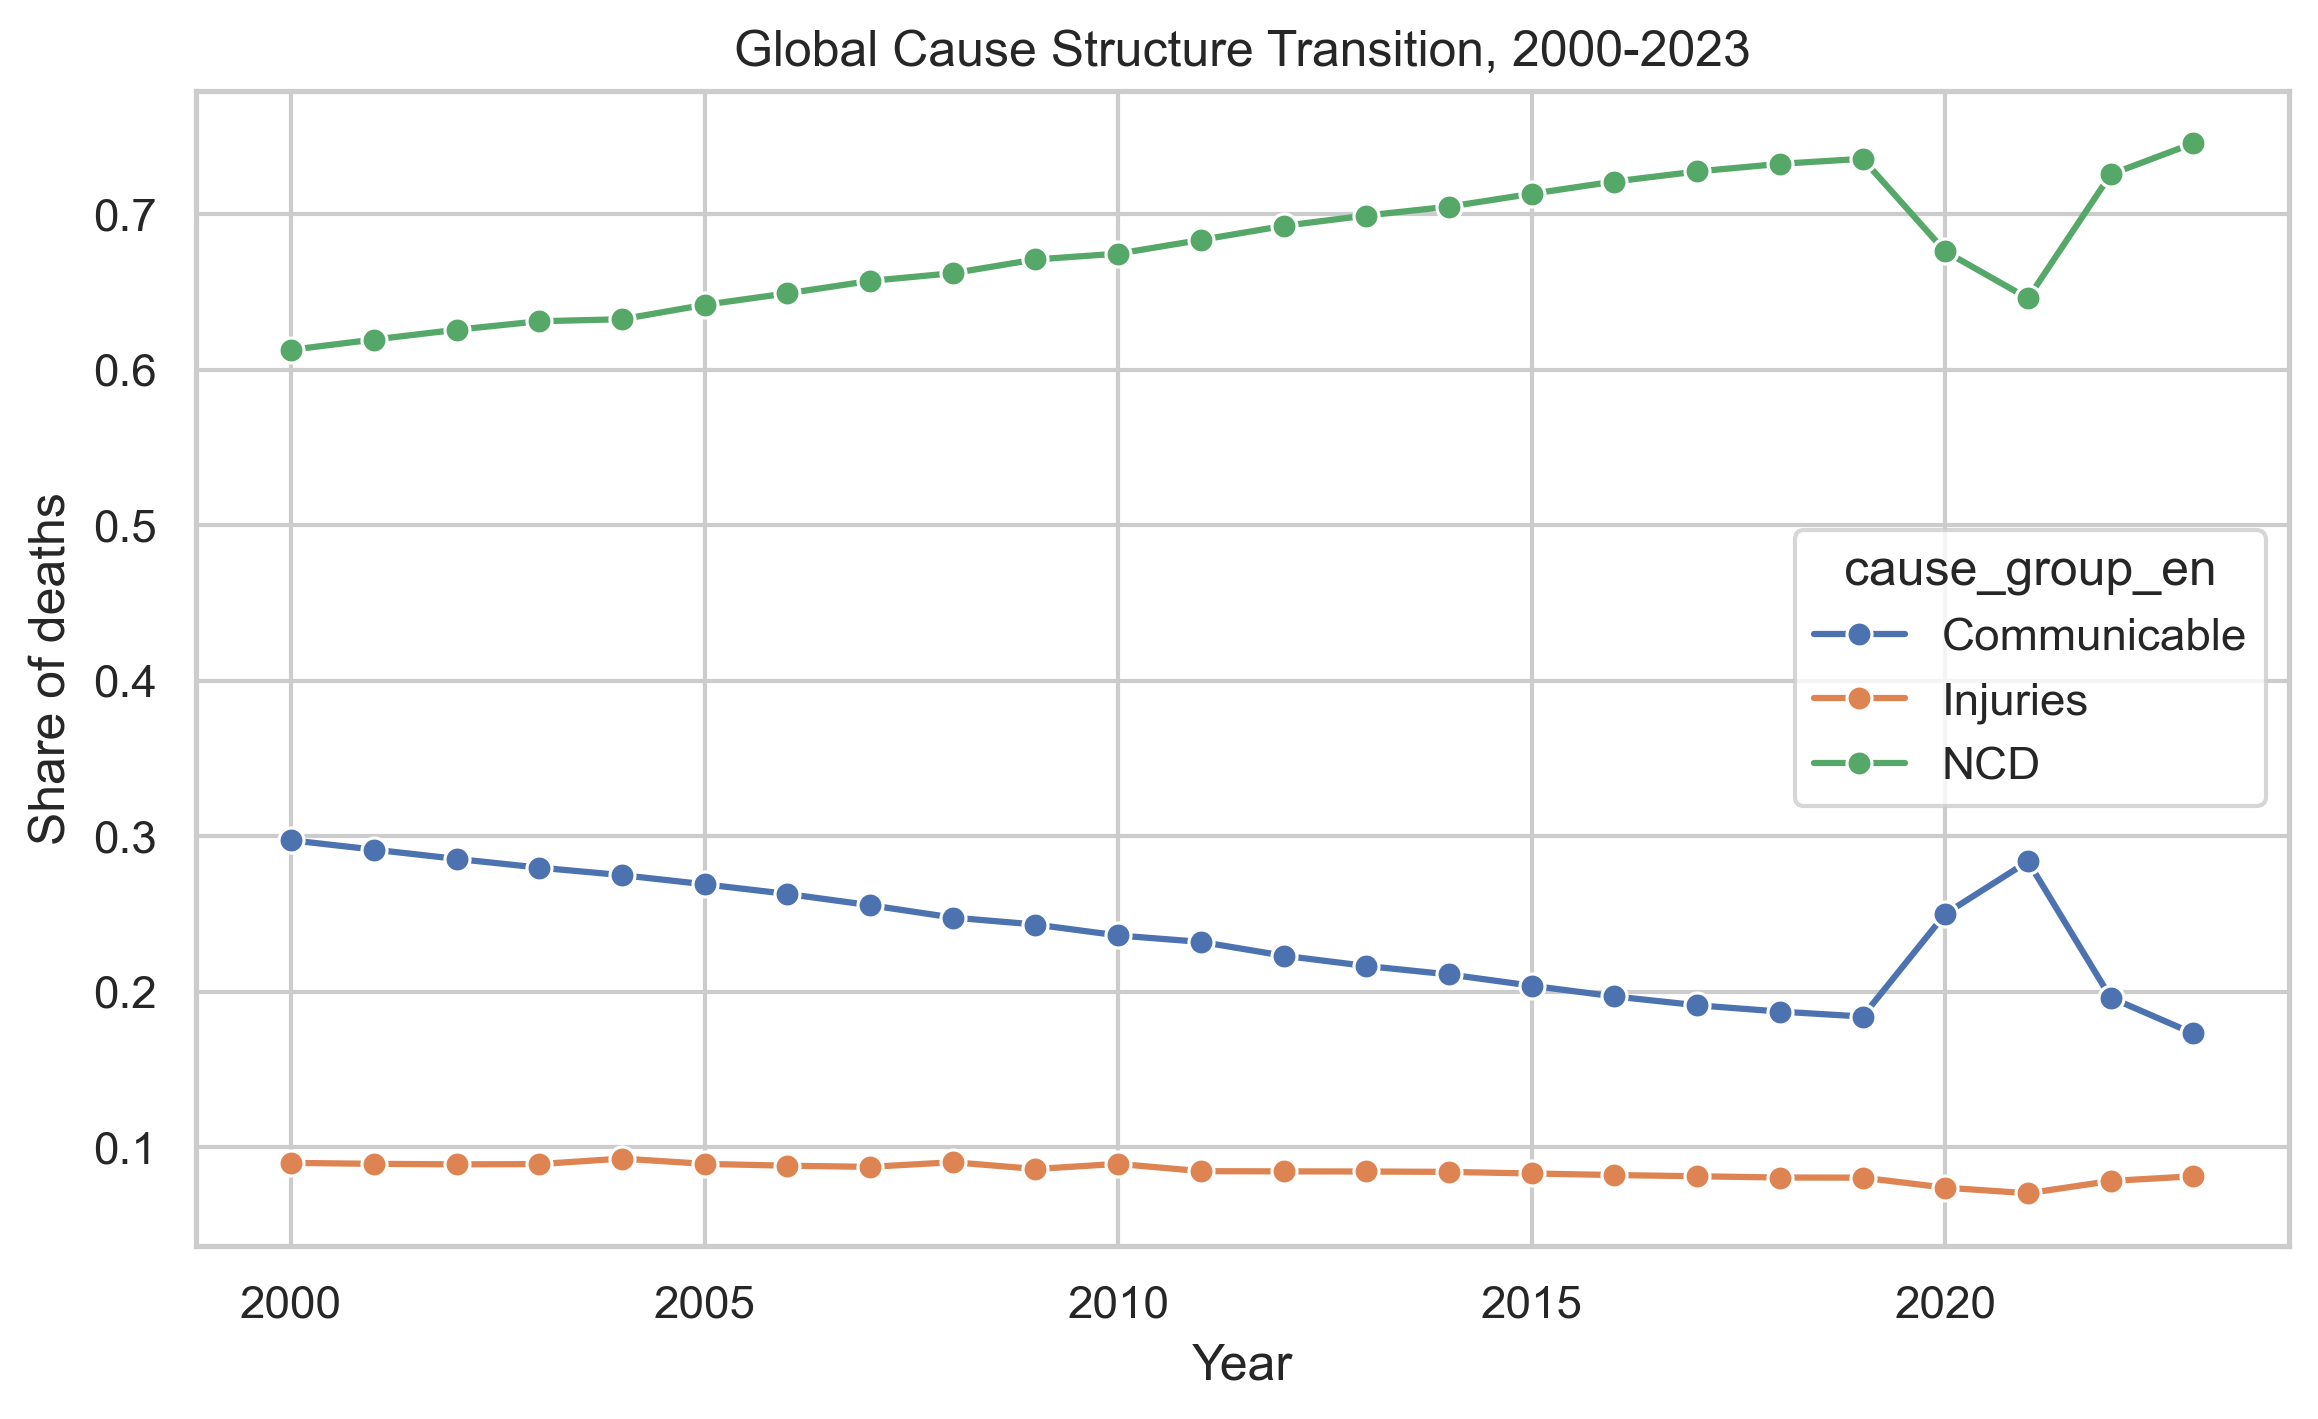
\includegraphics[width=0.82\textwidth]{figures/fig01_global_disease_transition.png}
    \caption{2000--2023 年全球疾病谱三大类结构变化}
    \label{fig:dim1-transition}
\end{figure}

\subsection{关键健康指标差异}
2023 年，日本的预期寿命最高，约为 84.0 岁；乍得最低，约为 53.0 岁。高寿命国家几乎都具有较高的非传染性疾病占比，原因不是“慢病更严重”，而是这些国家已经完成传染性疾病控制和人口转型，死亡结构更集中在高龄慢病。

\begin{tabular}{lrrr}
\toprule
country_name & life_expectancy & ncd_share & communicable_share \\
\midrule
Japan & 83.996 & 0.883 & 0.068 \\
Switzerland & 83.454 & 0.878 & 0.057 \\
Australia & 83.200 & 0.903 & 0.032 \\
Sweden & 83.110 & 0.898 & 0.048 \\
Spain & 83.083 & 0.885 & 0.058 \\
Ireland & 83.056 & 0.900 & 0.059 \\
Luxembourg & 83.046 & 0.872 & 0.058 \\
Italy & 82.900 & 0.888 & 0.055 \\
Singapore & 82.895 & 0.795 & 0.164 \\
New Zealand & 82.761 & 0.901 & 0.037 \\
\bottomrule
\end{tabular}


\begin{tabular}{lrrr}
\toprule
country_name & life_expectancy & ncd_share & communicable_share \\
\midrule
Chad & 52.997 & 0.256 & 0.664 \\
Lesotho & 53.036 & 0.371 & 0.524 \\
Nigeria & 53.633 & 0.338 & 0.583 \\
Central African Republic & 54.477 & 0.240 & 0.667 \\
South Sudan & 55.567 & 0.338 & 0.517 \\
Somalia, Fed. Rep. & 56.107 & 0.232 & 0.650 \\
Eswatini & 56.360 & 0.348 & 0.520 \\
Namibia & 58.059 & 0.408 & 0.428 \\
Côte d'Ivoire & 58.916 & 0.355 & 0.547 \\
Guinea & 58.985 & 0.377 & 0.538 \\
\bottomrule
\end{tabular}


图 \ref{fig:dim1-scatter} 进一步显示，在 2023 年截面上，传染性疾病占比越高，预期寿命通常越低。

\begin{figure}[H]
    \centering
    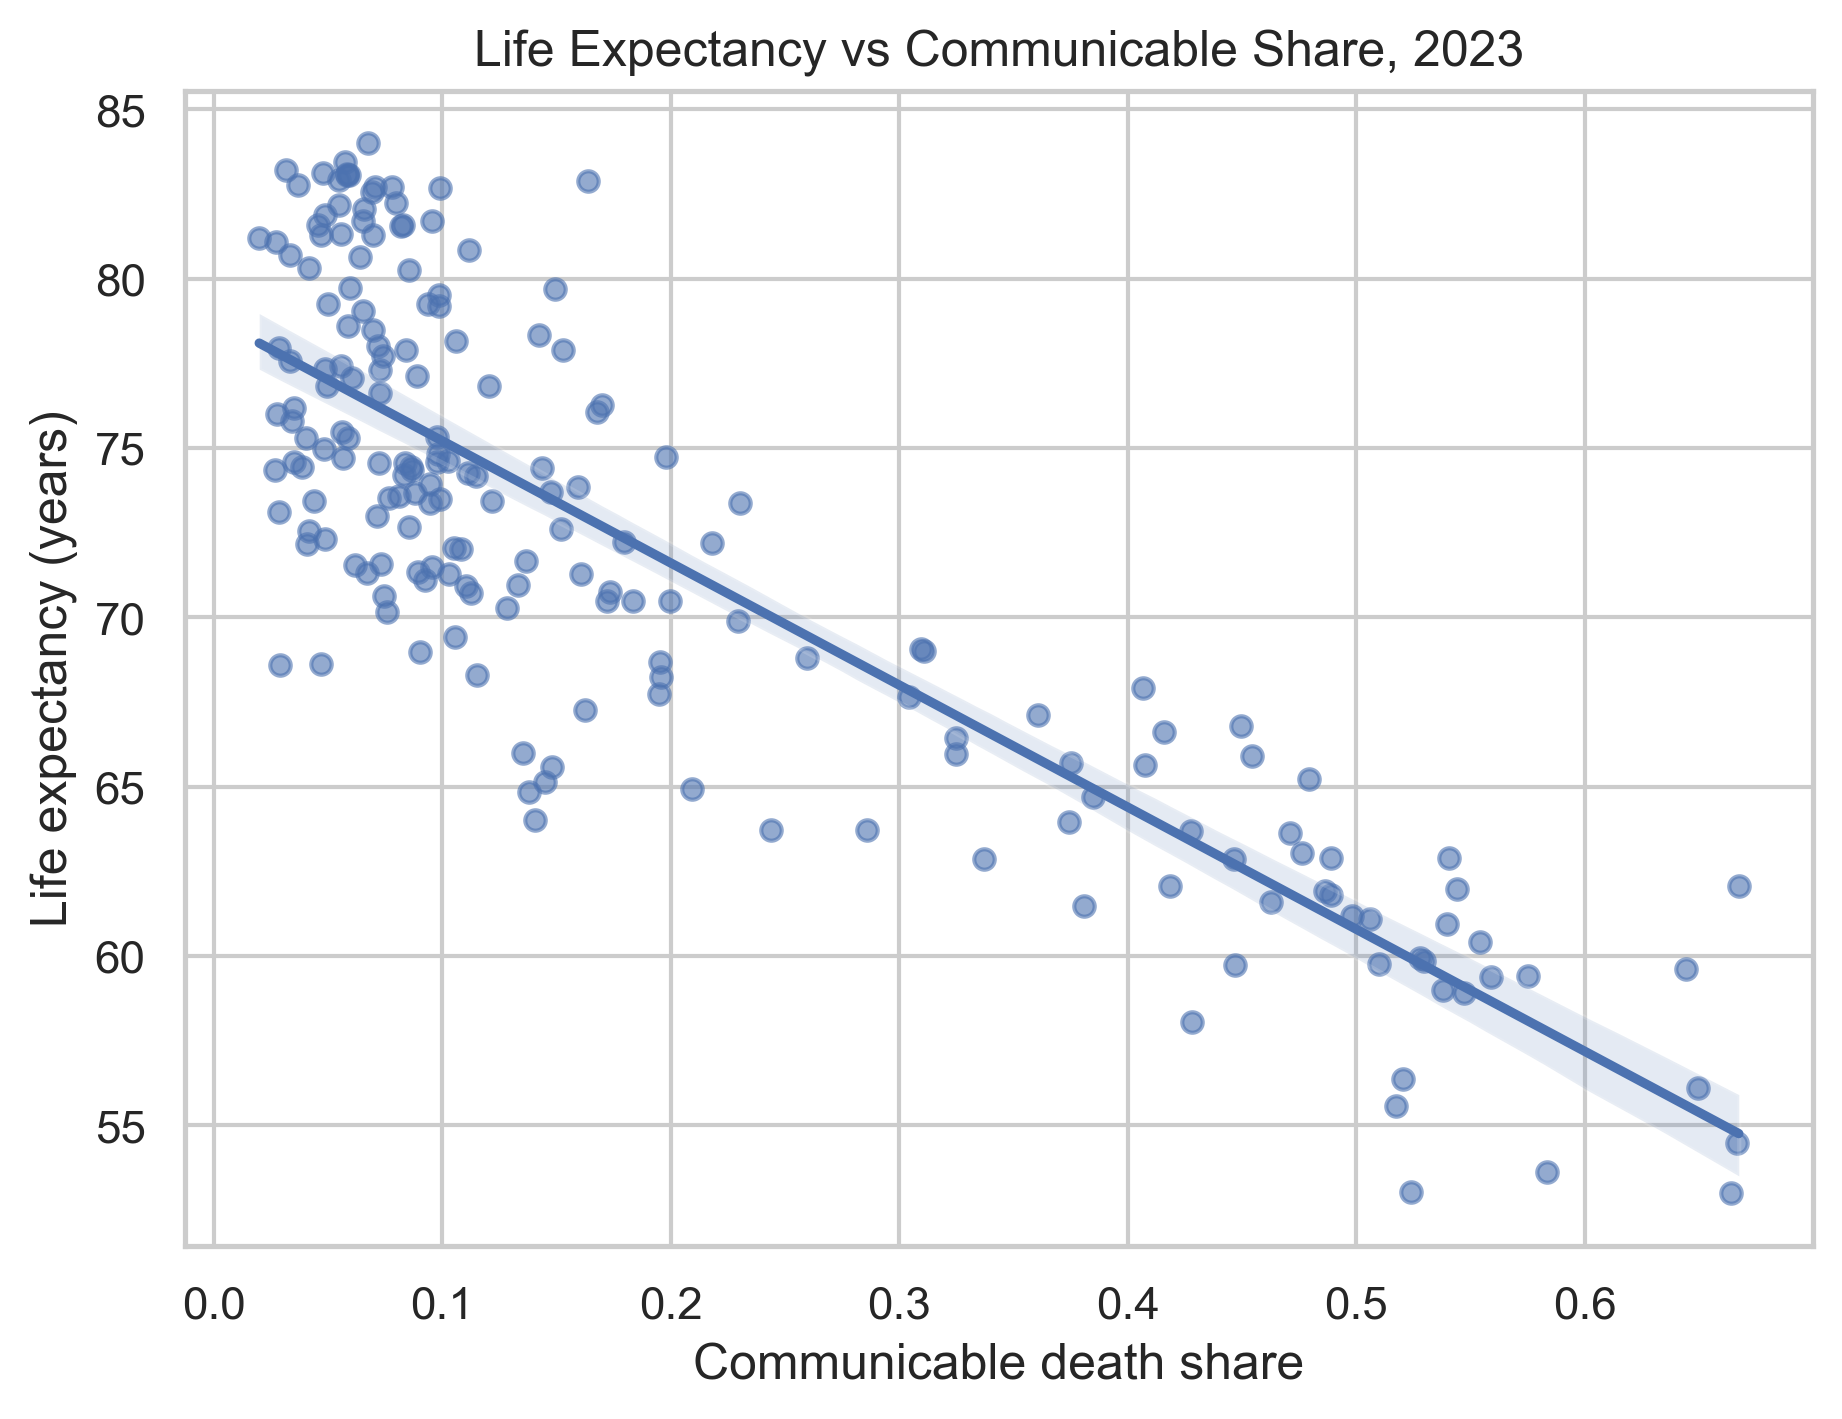
\includegraphics[width=0.72\textwidth]{figures/fig02_life_expectancy_vs_communicable_share.png}
    \caption{2023 年传染性疾病死亡占比与预期寿命关系}
    \label{fig:dim1-scatter}
\end{figure}

\subsection{解释与预测}
在最新年份的截面回归中，人均 GDP 对寿命呈显著正相关，模型 $R^2$ 为 0.906，说明经济基础仍然是寿命差异的重要背景变量。卫生支出占 GDP 比重、供水与卫生条件的方向与预期一致，但在控制多变量后显著性下降，这表明这些因素之间存在较强共线性或发展阶段耦合关系。

\begin{tabular}{lrr}
\toprule
variable & coef & p_value \\
\midrule
const & 50.051 & 0.001 \\
log_gdp_per_capita & 1.879 & 0.003 \\
health_exp_pct_gdp & 0.292 & 0.129 \\
physicians_per_1000 & -0.094 & 0.820 \\
basic_water_pct & -0.036 & 0.629 \\
basic_sanitation_pct & 0.025 & 0.575 \\
communicable_share & -15.017 & 0.355 \\
ncd_share & 10.975 & 0.469 \\
\bottomrule
\end{tabular}


在预测部分，项目对中、美、印、巴西、南非和德国等代表国家的寿命与非传染性疾病占比进行线性趋势外推，结果作为“政策情景之外的基线延续”。

\begin{figure}[H]
    \centering
    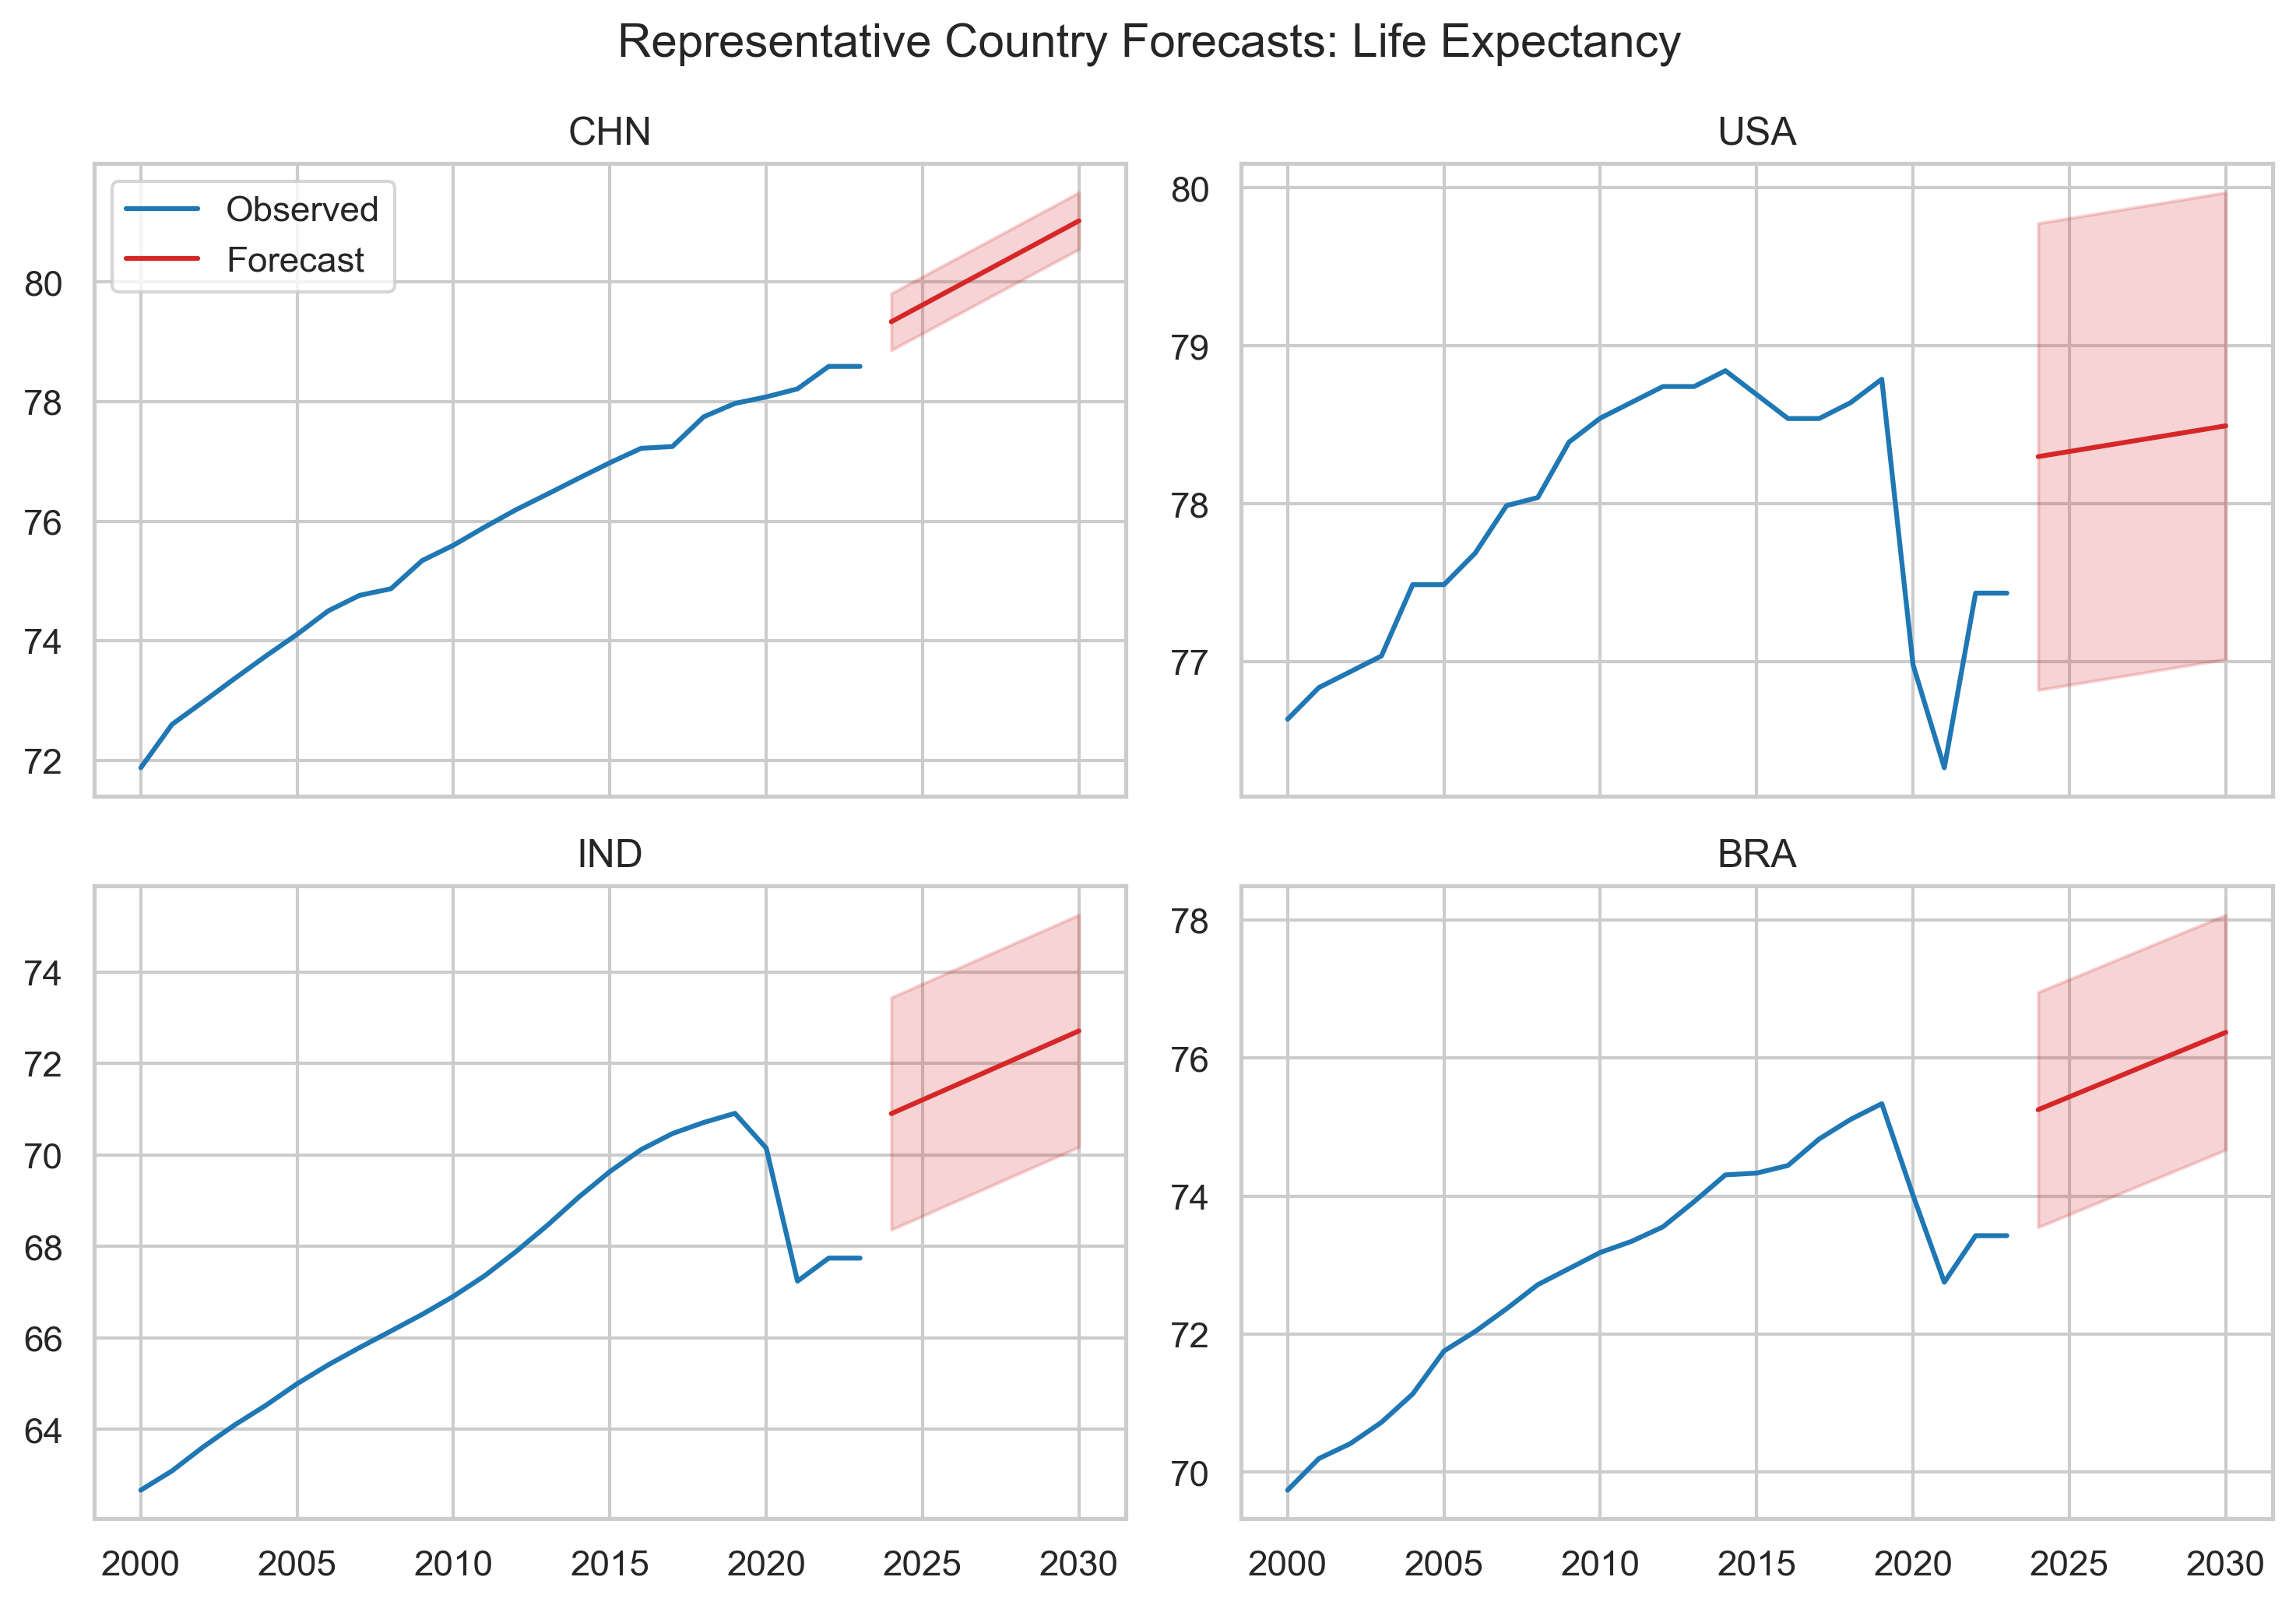
\includegraphics[width=0.88\textwidth]{figures/fig03_dim1_forecasts.png}
    \caption{代表国家预期寿命预测}
\end{figure}

\section{Dimension 2：风险因素归因与干预优先级}
\subsection{全球主要风险因素归因死亡}
2023 年，全球归因死亡规模最大的风险因素是高血压，其后是饮食风险、高血糖、空气污染等。这个排序说明慢病风险管理已成为全球公共卫生的中心议题。

\begin{figure}[H]
    \centering
    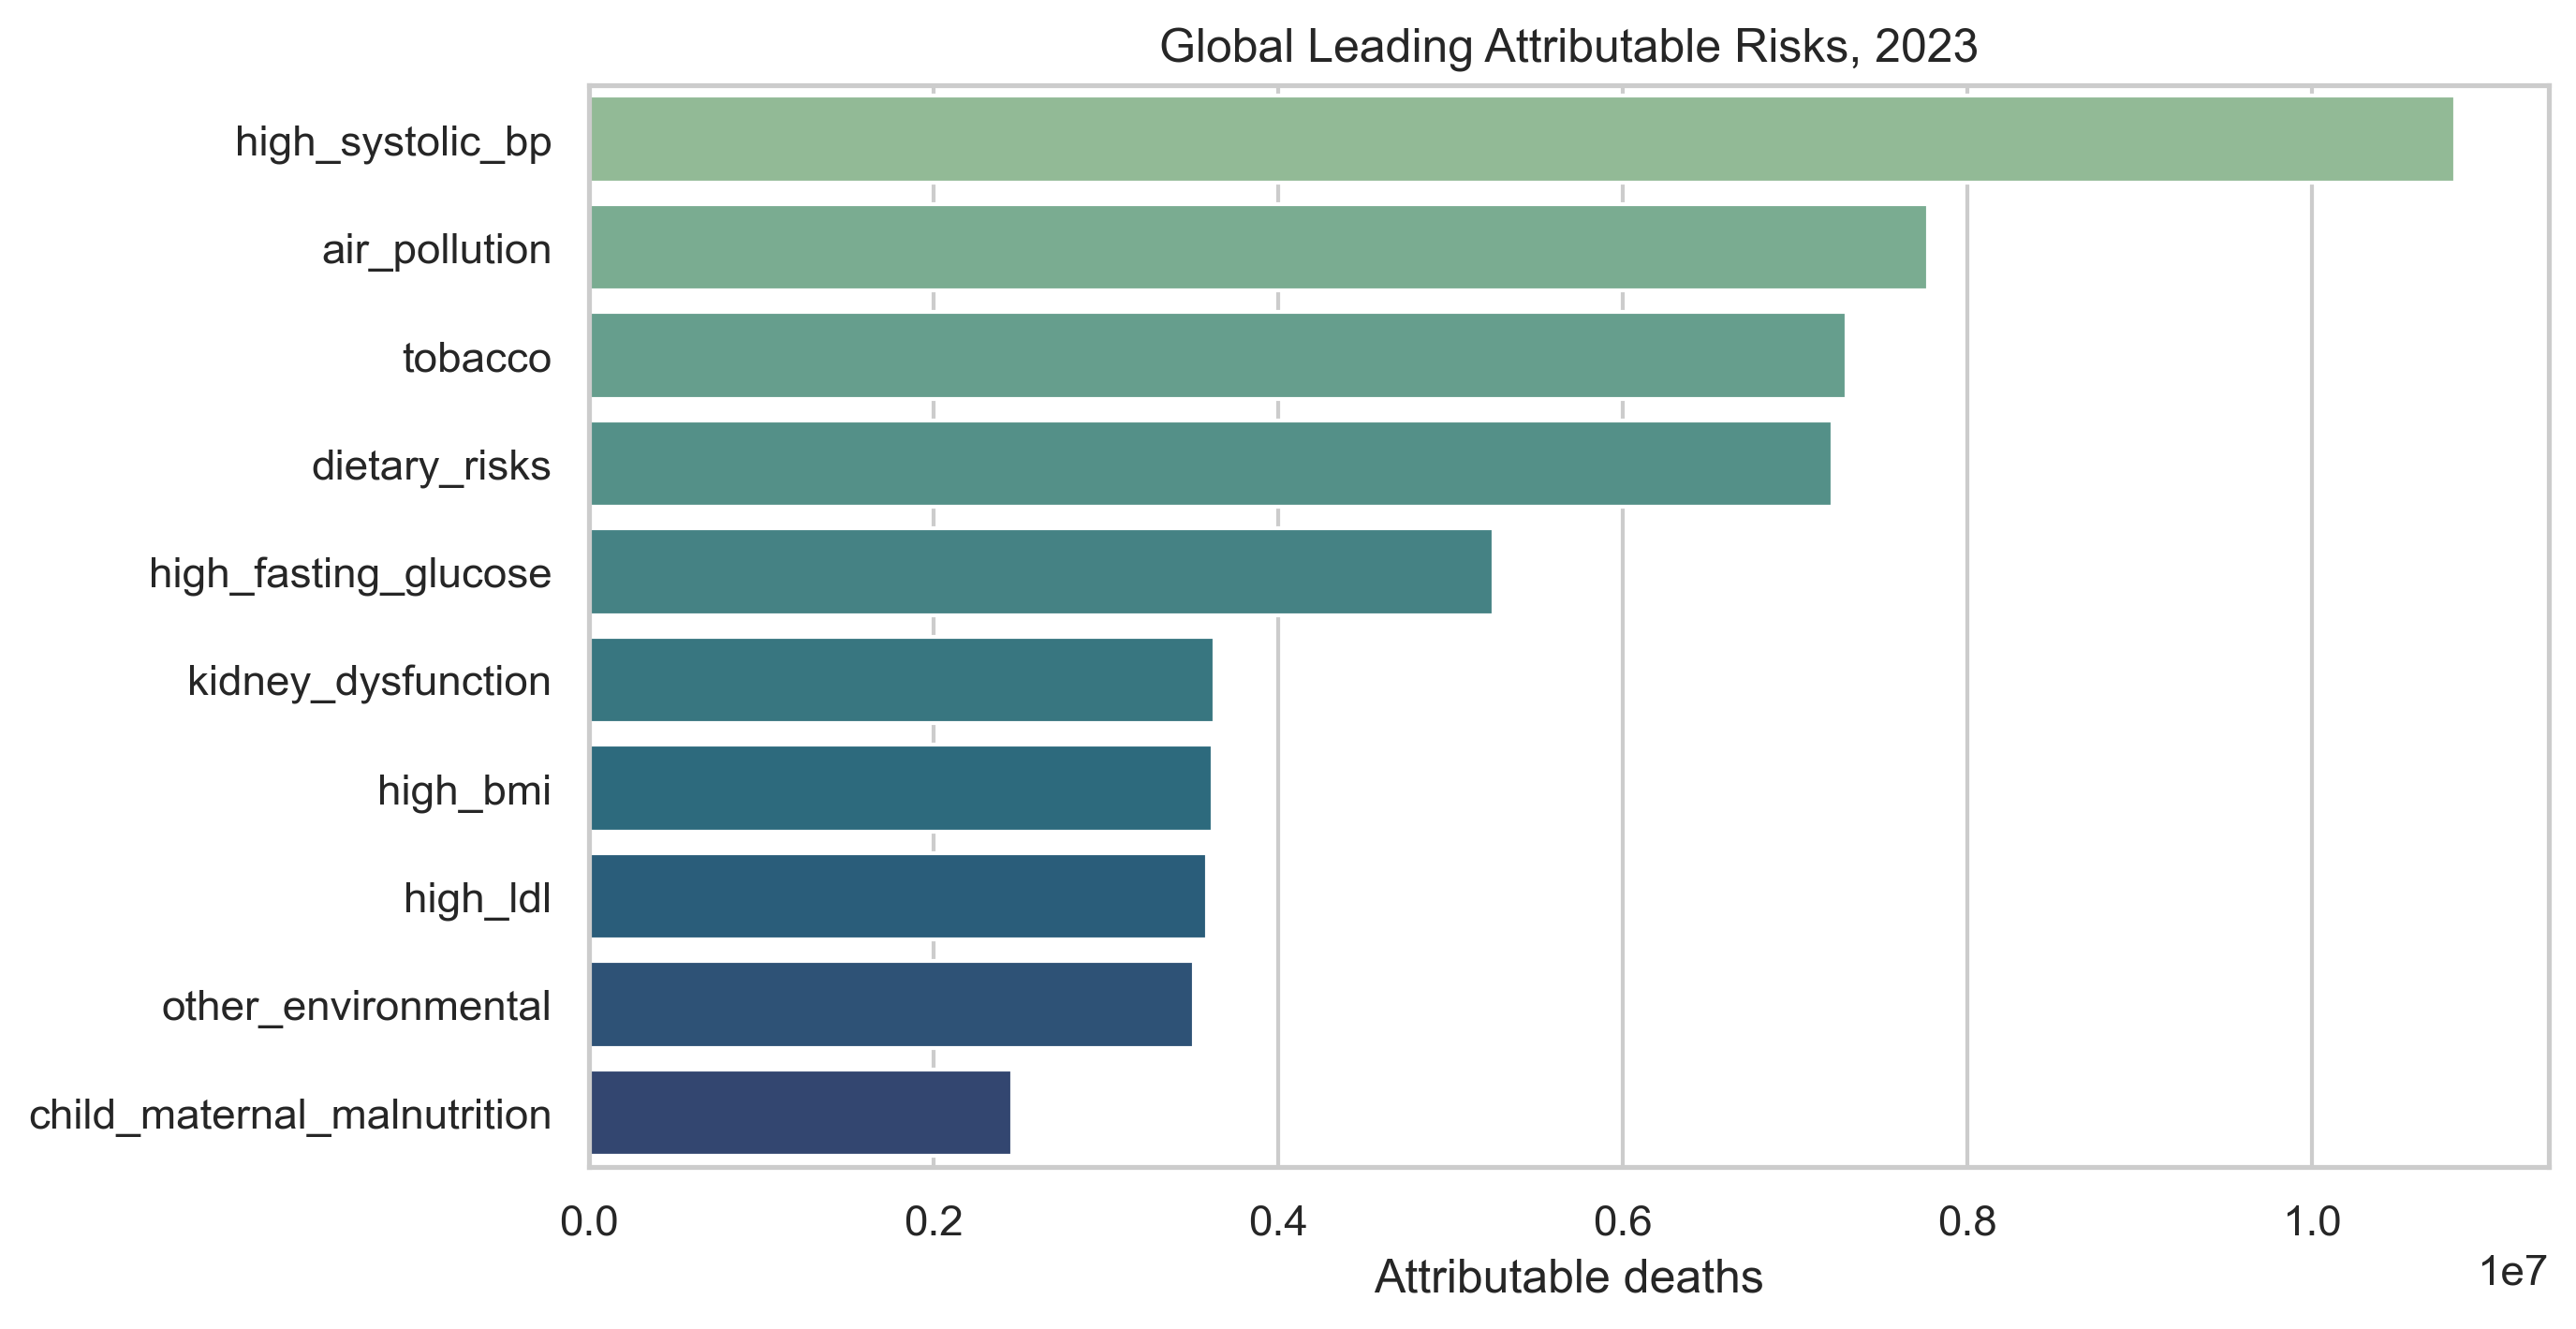
\includegraphics[width=0.8\textwidth]{figures/fig04_dim2_global_risk_bar.png}
    \caption{2023 年全球主要风险因素归因死亡规模}
\end{figure}

\subsection{地区差异}
图 \ref{fig:dim2-heatmap} 表明，WHO 各地区在主要风险因素上的“主次矛盾”并不相同。EURO、AMRO、WPRO 和 EMRO 的首要风险均为高血压；SEARO 的空气污染问题更突出；AFRO 的首要风险则是儿童和孕产妇营养不良。
考虑到 provided 风险数据只有“所有原因”口径，本项目没有伪造疾病特异性链路，而是额外导出了“风险因素 $\rightarrow$ WHO 地区 $\rightarrow$ 归因死亡规模”的交互式 Sankey 资产，用于展示不同风险在全球地区之间的流向结构。

\begin{figure}[H]
    \centering
    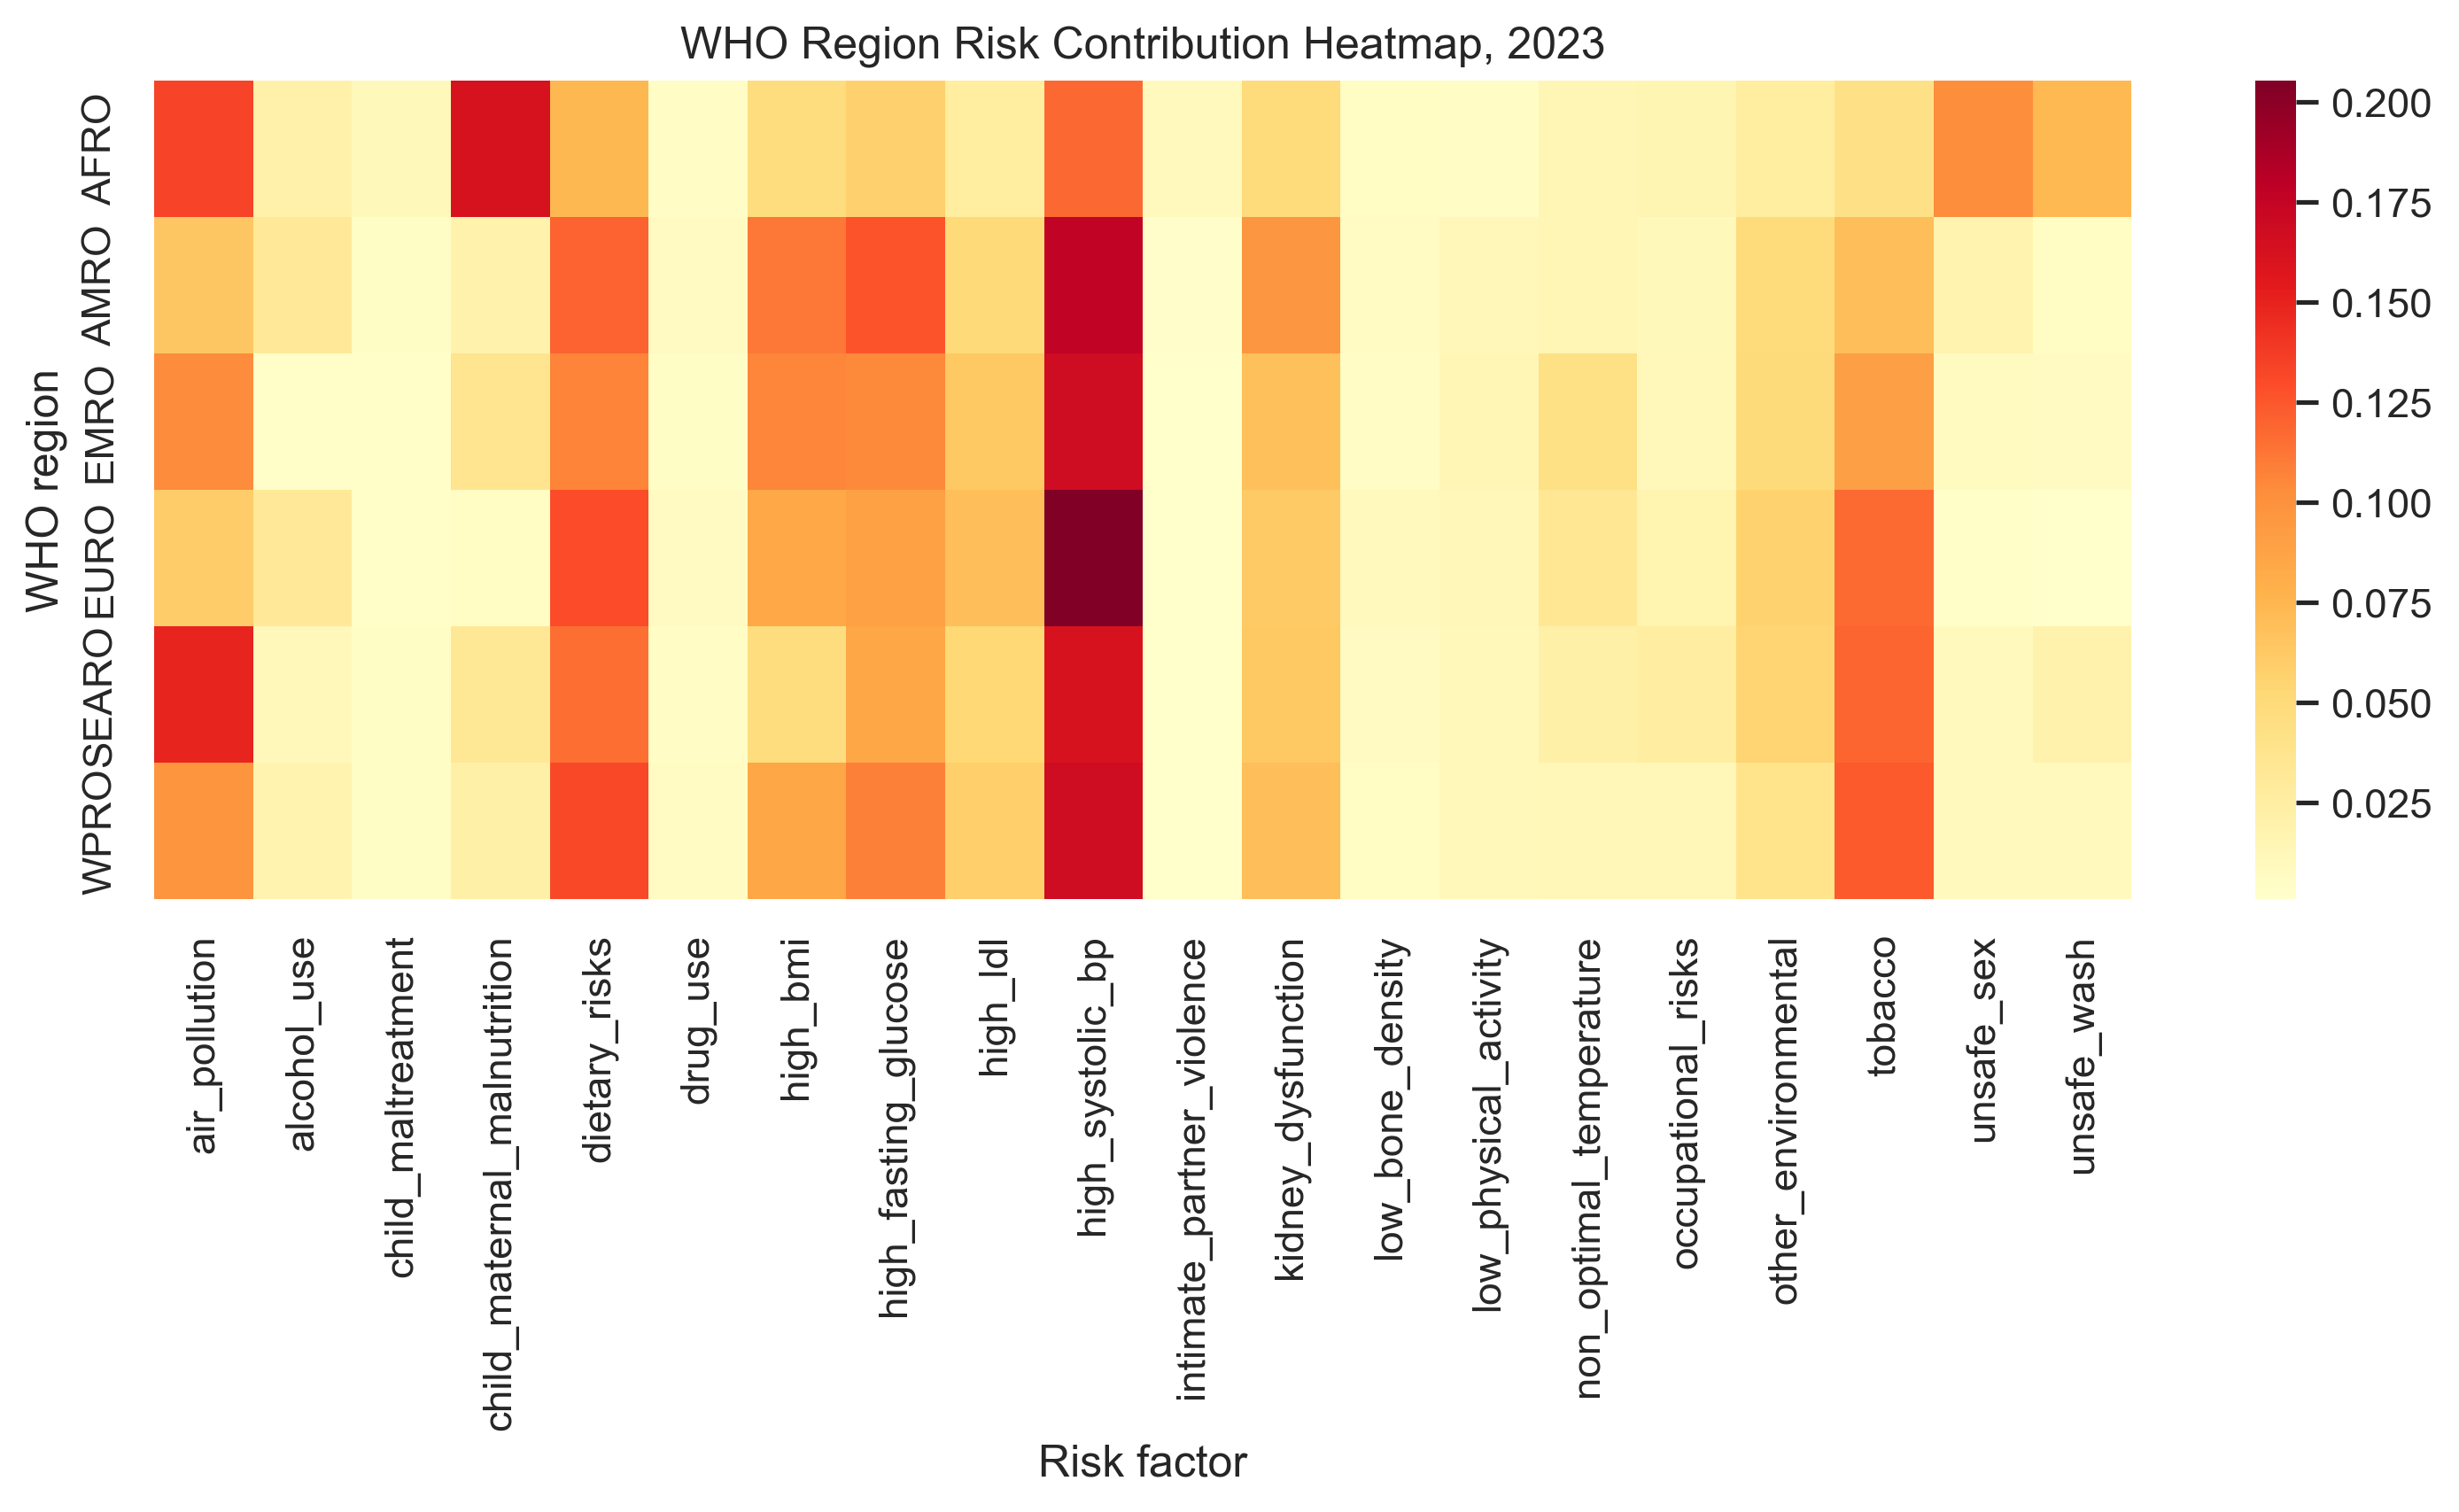
\includegraphics[width=0.95\textwidth]{figures/fig05_dim2_region_heatmap.png}
    \caption{2023 年各 WHO 地区风险归因占比热力图}
    \label{fig:dim2-heatmap}
\end{figure}

\begin{tabular}{lllrllrl}
\toprule
who_region & primary_risk & primary_risk_code & primary_share & secondary_risk & secondary_risk_code & secondary_share & recommended_intervention \\
\midrule
EURO & 高血压 & high_systolic_bp & 0.205 & 饮食风险 & dietary_risks & 0.130 & 基层筛查、高血压规范管理和药物可及性 \\
AMRO & 高血压 & high_systolic_bp & 0.177 & 高血糖 & high_fasting_glucose & 0.127 & 基层筛查、高血压规范管理和药物可及性 \\
WPRO & 高血压 & high_systolic_bp & 0.169 & 饮食风险 & dietary_risks & 0.131 & 基层筛查、高血压规范管理和药物可及性 \\
EMRO & 高血压 & high_systolic_bp & 0.168 & 饮食风险 & dietary_risks & 0.107 & 基层筛查、高血压规范管理和药物可及性 \\
SEARO & 高血压 & high_systolic_bp & 0.162 & 空气污染 & air_pollution & 0.149 & 基层筛查、高血压规范管理和药物可及性 \\
AFRO & 儿童和孕产妇营养不良 & child_maternal_malnutrition & 0.162 & 空气污染 & air_pollution & 0.134 & 孕产妇营养补充、儿童早期营养支持 \\
\bottomrule
\end{tabular}


\subsection{未来情景与干预建议}
在基准情景下，全球主要风险归因死亡仍会延续既有趋势。温和干预假设到 2030 年使总归因死亡较基准下降约 10\%，强化干预情景则下降约 20\%。这类情景不是为了给出单点真值，而是为“政策力度差异会带来怎样的量级变化”提供量化参考。

\begin{figure}[H]
    \centering
    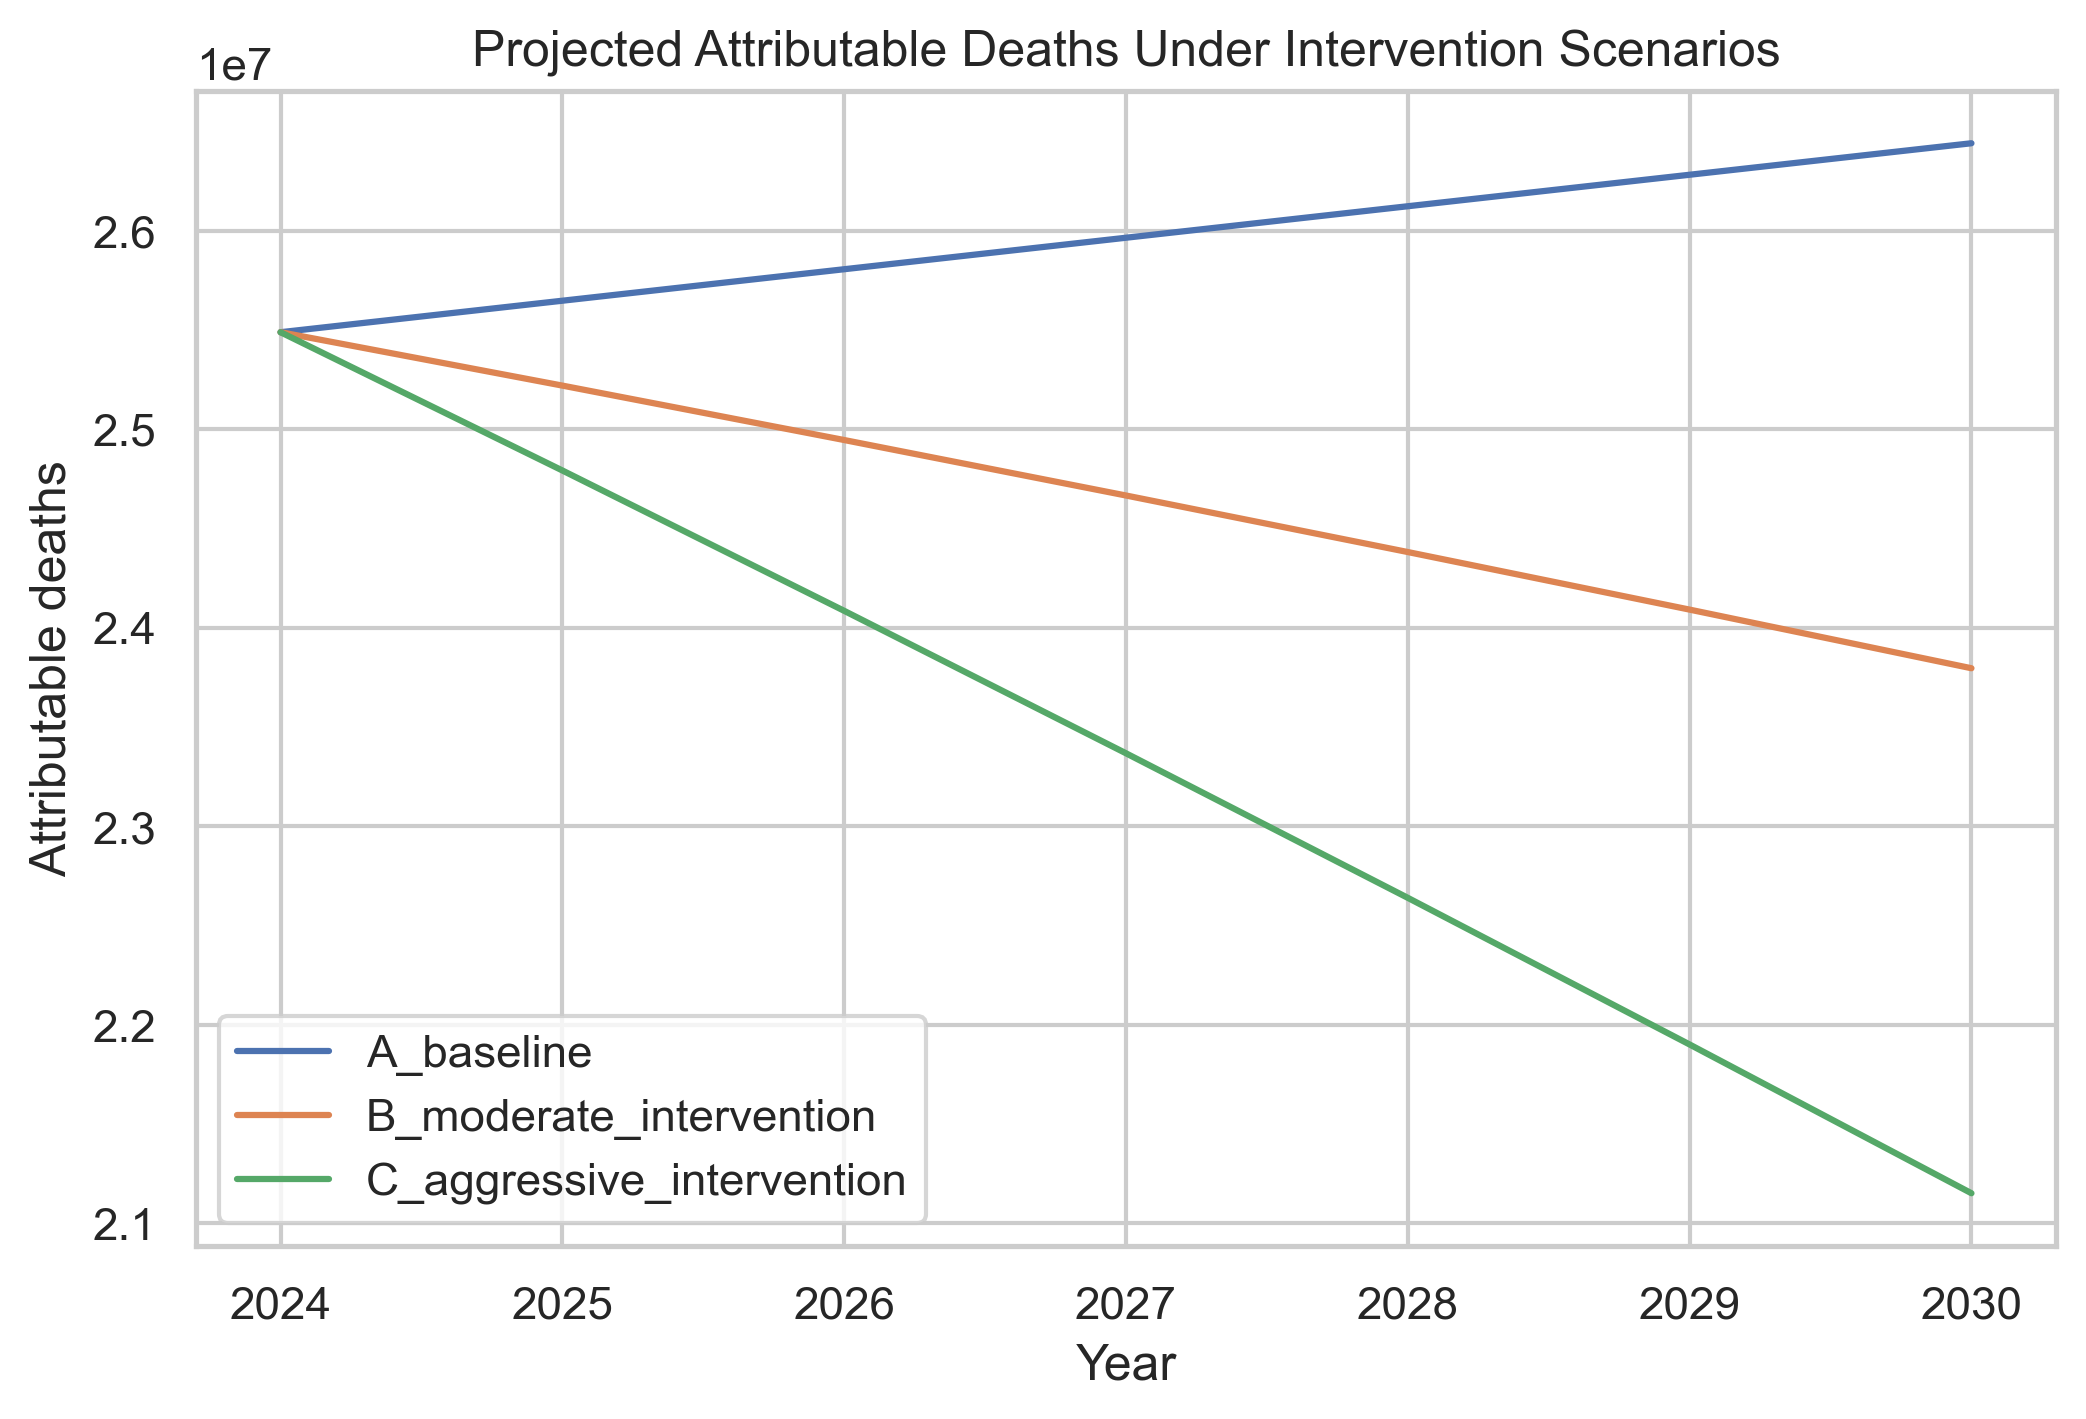
\includegraphics[width=0.78\textwidth]{figures/fig06_dim2_scenarios.png}
    \caption{不同干预情景下全球主要风险归因死亡变化}
\end{figure}

结合各地区主导风险，项目给出如下优先干预原则：
\begin{itemize}[leftmargin=1.5em]
    \item 高血压主导地区：优先做基层筛查、规范管理与药物可及性提升；
    \item 空气污染主导地区：优先做清洁能源、工业减排和空气质量治理；
    \item 儿童和孕产妇营养不良主导地区：优先补足孕产妇和儿童早期营养支持体系。
\end{itemize}

\section{Dimension 3：卫生资源配置与优化见解}
\subsection{资源缺口识别}
资源缺口指标通过“实际资源投入指数减理论需求指数”得到。2023 年，索马里、乍得、尼日利亚、尼日尔和马里等国家处于最严重短缺组，且几乎集中在 AFRO 地区，反映出资源稀缺与疾病负担高位叠加的结构性问题。

\begin{tabular}{llllrrrrll}
\toprule
iso3 & country_name & who_region & wb_income & year & actual_resource_index & theoretical_need_index & gap & gap_grade & gap_grade_en \\
\midrule
SOM & Somalia, Fed. Rep. & AFRO & LIC & 2023 & -0.957 & 2.623 & -3.581 & E_严重不足 & E_critical_shortage \\
TCD & Chad & AFRO & LIC & 2023 & -0.857 & 2.661 & -3.518 & E_严重不足 & E_critical_shortage \\
NER & Niger & AFRO & LIC & 2023 & -0.929 & 2.451 & -3.380 & E_严重不足 & E_critical_shortage \\
NGA & Nigeria & AFRO & LMC & 2023 & -0.744 & 2.629 & -3.373 & E_严重不足 & E_critical_shortage \\
CAF & Central African Republic & AFRO & LIC & 2023 & -0.436 & 2.689 & -3.125 & E_严重不足 & E_critical_shortage \\
MLI & Mali & AFRO & LIC & 2023 & -0.902 & 2.180 & -3.081 & E_严重不足 & E_critical_shortage \\
GIN & Guinea & AFRO & LMC & 2023 & -0.854 & 2.192 & -3.046 & E_严重不足 & E_critical_shortage \\
SSD & South Sudan & AFRO & LIC & 2023 & -0.678 & 2.325 & -3.002 & E_严重不足 & E_critical_shortage \\
SLE & Sierra Leone & AFRO & LIC & 2023 & -0.593 & 2.408 & -3.001 & E_严重不足 & E_critical_shortage \\
BEN & Benin & AFRO & LMC & 2023 & -0.993 & 1.879 & -2.872 & E_严重不足 & E_critical_shortage \\
CIV & Côte d'Ivoire & AFRO & LMC & 2023 & -0.879 & 1.814 & -2.693 & E_严重不足 & E_critical_shortage \\
GNQ & Equatorial Guinea & AFRO & UMC & 2023 & -0.918 & 1.746 & -2.664 & E_严重不足 & E_critical_shortage \\
COD & Congo, Democratic Republic of & AFRO & LIC & 2023 & -0.822 & 1.812 & -2.635 & E_严重不足 & E_critical_shortage \\
CMR & Cameroon & AFRO & LMC & 2023 & -0.848 & 1.664 & -2.512 & E_严重不足 & E_critical_shortage \\
AGO & Angola & AFRO & LMC & 2023 & -0.939 & 1.510 & -2.450 & E_严重不足 & E_critical_shortage \\
\bottomrule
\end{tabular}


\subsection{投入--产出四象限}
图 \ref{fig:dim3-quadrant} 给出 2023 年各国投入--产出四象限。共有 26 个国家落入“低投入--高产出”象限，这些国家在资源受限条件下仍保持相对较好的健康结果，应作为经验总结对象；相反，“高投入--低产出”地区更需要关注治理效率与投入结构。

\begin{figure}[H]
    \centering
    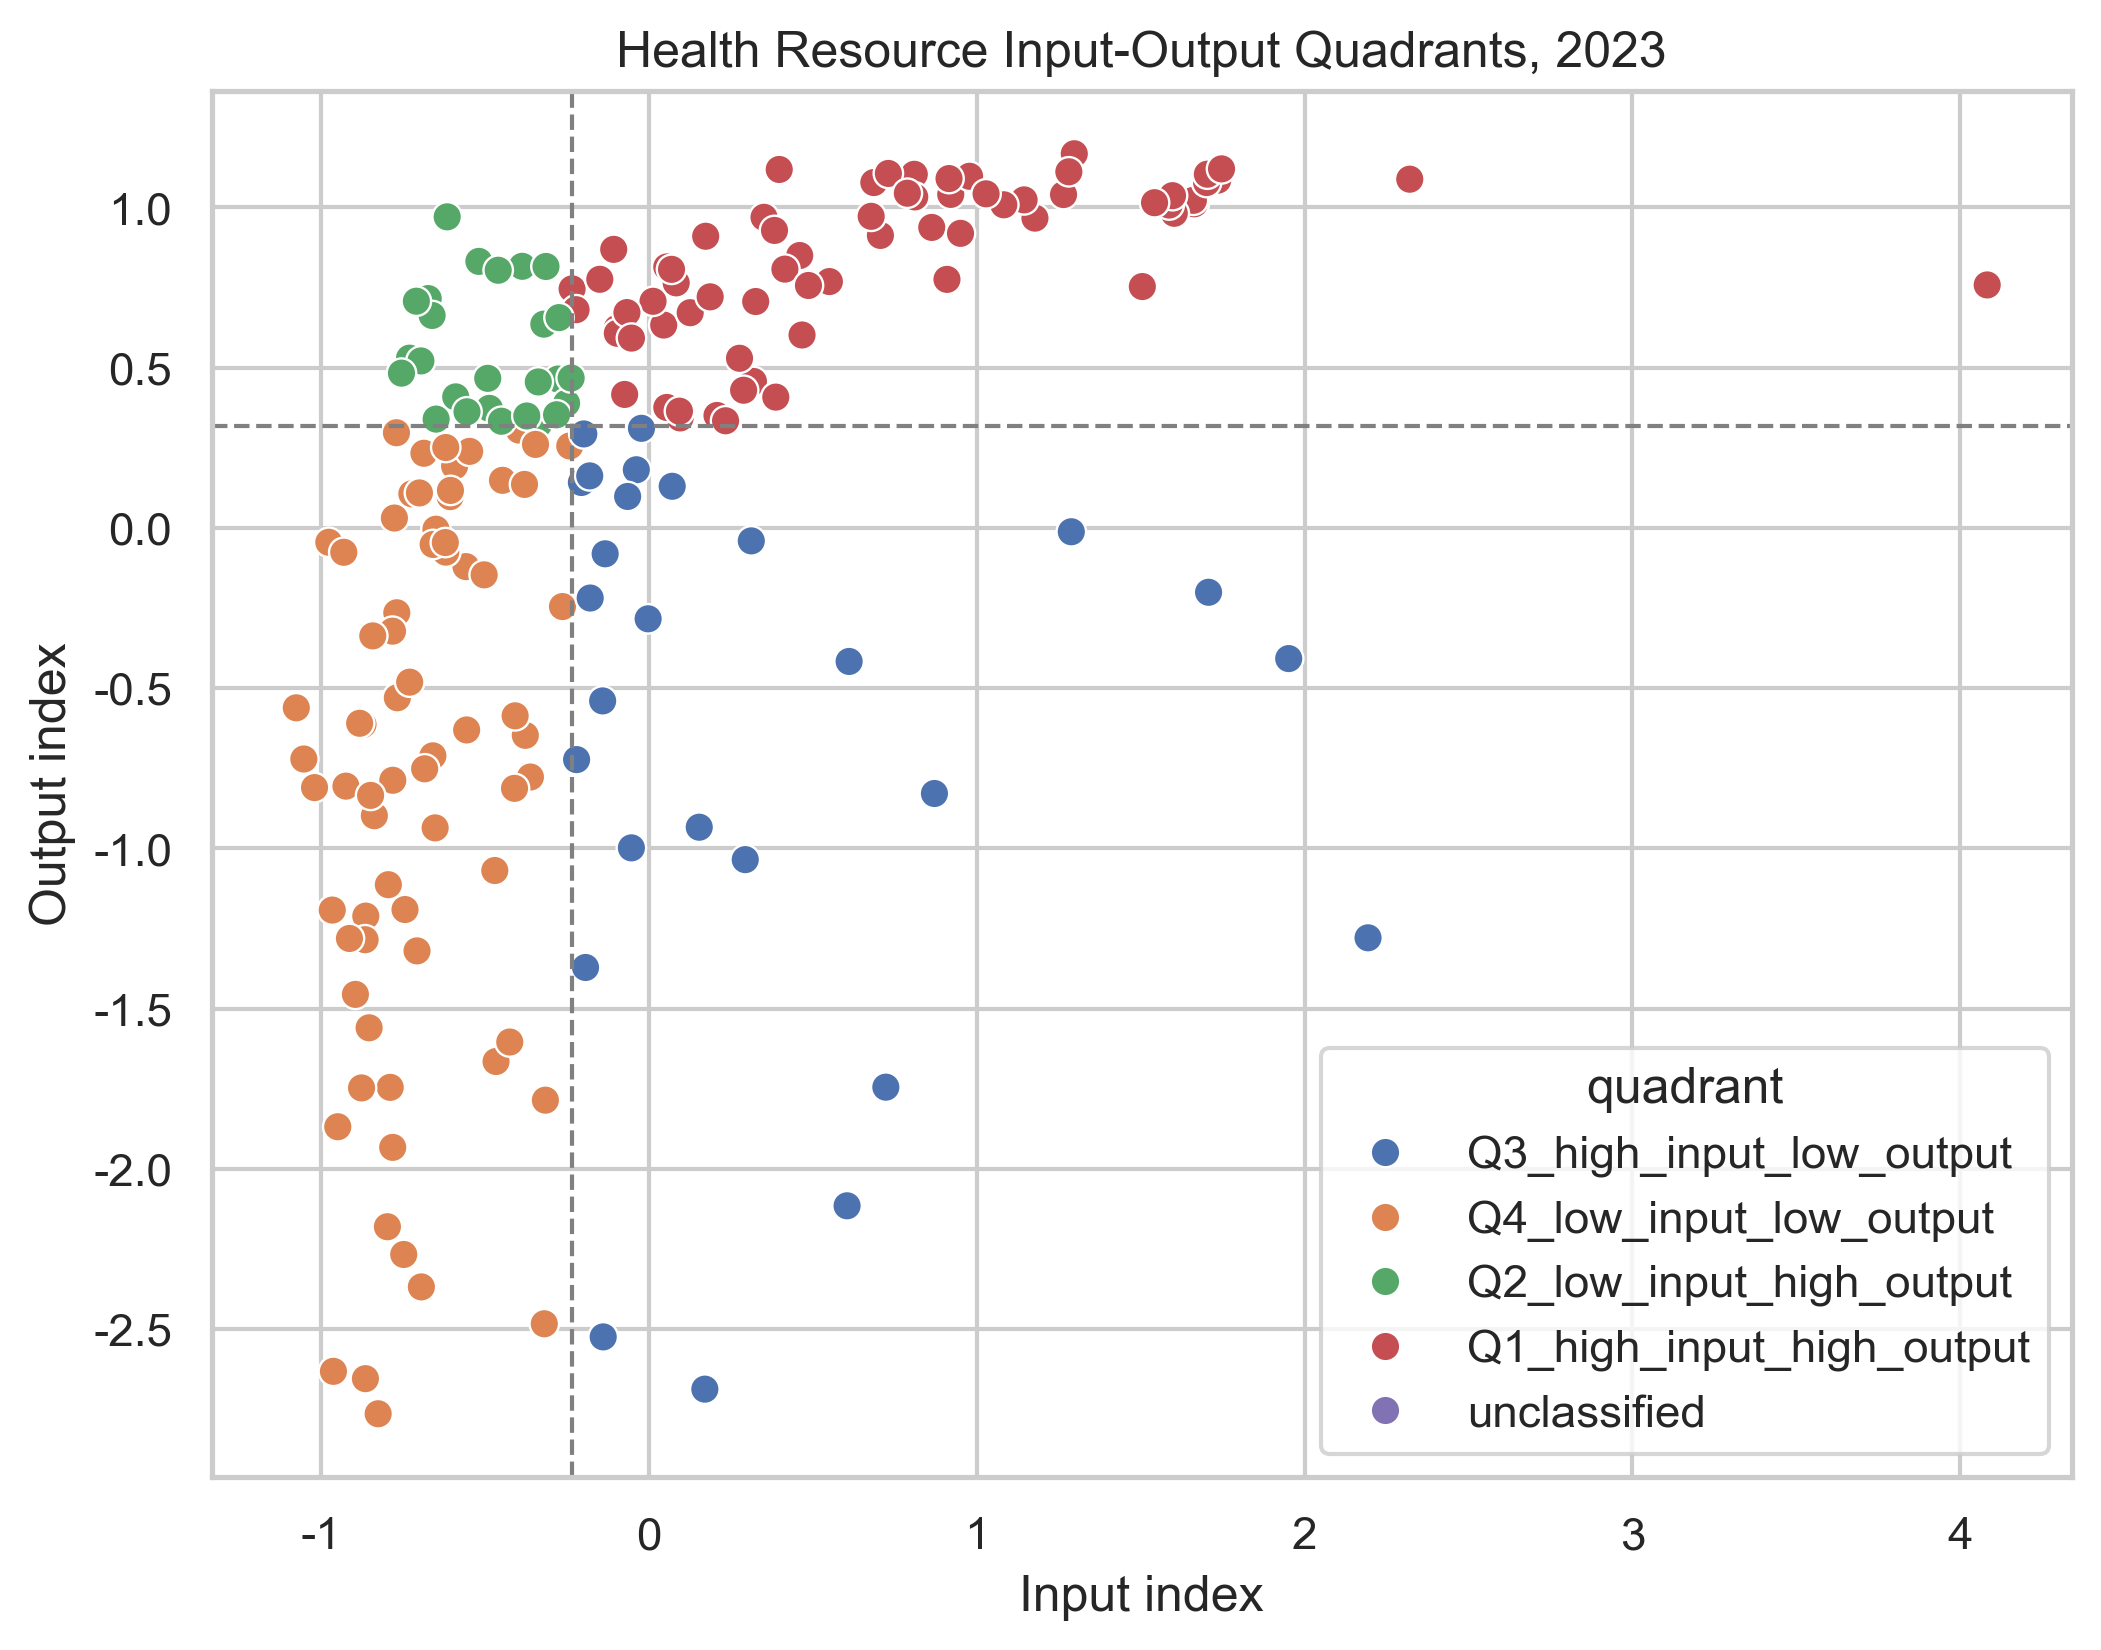
\includegraphics[width=0.78\textwidth]{figures/fig07_dim3_quadrant.png}
    \caption{2023 年各国卫生资源投入--产出四象限}
    \label{fig:dim3-quadrant}
\end{figure}

\subsection{再分配模拟}
本项目在总预算不变、单国人均卫生支出变动受上下界约束的前提下，构建了需求加权的对数收益优化模型。结果显示，阿富汗、毛里塔尼亚、马达加斯加、马里、莫桑比克等高需求国家获得更高的优先度，而一些需求相对较低但当前支出较高的国家应更多承担再平衡空间。

\begin{tabular}{llrrrrrr}
\toprule
iso3 & country_name & health_exp_per_capita & theoretical_need & current & optimal & change & change_pct \\
\midrule
AFG & Afghanistan & 80.652 & 1.167 & 80.652 & 96.782 & 16.130 & 20.000 \\
BEN & Benin & 33.882 & 1.879 & 33.882 & 40.659 & 6.776 & 20.000 \\
GRD & Grenada & 521.237 & -0.410 & 521.237 & 625.485 & 104.247 & 20.000 \\
IDN & Indonesia & 127.444 & 0.065 & 127.444 & 152.933 & 25.489 & 20.000 \\
CIV & Côte d'Ivoire & 86.152 & 1.814 & 86.152 & 103.383 & 17.230 & 20.000 \\
LCA & St. Lucia & 644.803 & -0.285 & 644.803 & 773.763 & 128.961 & 20.000 \\
MUS & Mauritius & 590.936 & -0.403 & 590.936 & 709.123 & 118.187 & 20.000 \\
BWA & Botswana & 477.833 & 0.859 & 477.833 & 573.399 & 95.567 & 20.000 \\
PNG & Papua New Guinea & 81.114 & 0.731 & 81.114 & 97.336 & 16.223 & 20.000 \\
STP & São Tomé and Principe & 180.334 & -0.024 & 180.334 & 216.400 & 36.067 & 20.000 \\
SWZ & Eswatini & 283.883 & 1.496 & 283.883 & 340.660 & 56.777 & 20.000 \\
TCD & Chad & 40.170 & 2.661 & 40.170 & 48.204 & 8.034 & 20.000 \\
PSE & West Bank and Gaza & 350.638 & -0.470 & 350.638 & 420.766 & 70.128 & 20.000 \\
TUV & Tuvalu & 1084.670 & 0.077 & 1084.670 & 1301.603 & 216.934 & 20.000 \\
TKM & Turkmenistan & 579.155 & 0.320 & 579.155 & 694.985 & 115.831 & 20.000 \\
\bottomrule
\end{tabular}


\subsection{中国补充分析}
对中国省级数据的补充分析显示，东部与人口大省在卫生人员数量和卫生机构数量上的规模优势更加明显。图 \ref{fig:china-trends} 给出重点省份的 2005--2024 年趋势，用于补充赛题要求中“可在一国内部讨论资源配置差异”的视角。

\begin{figure}[H]
    \centering
    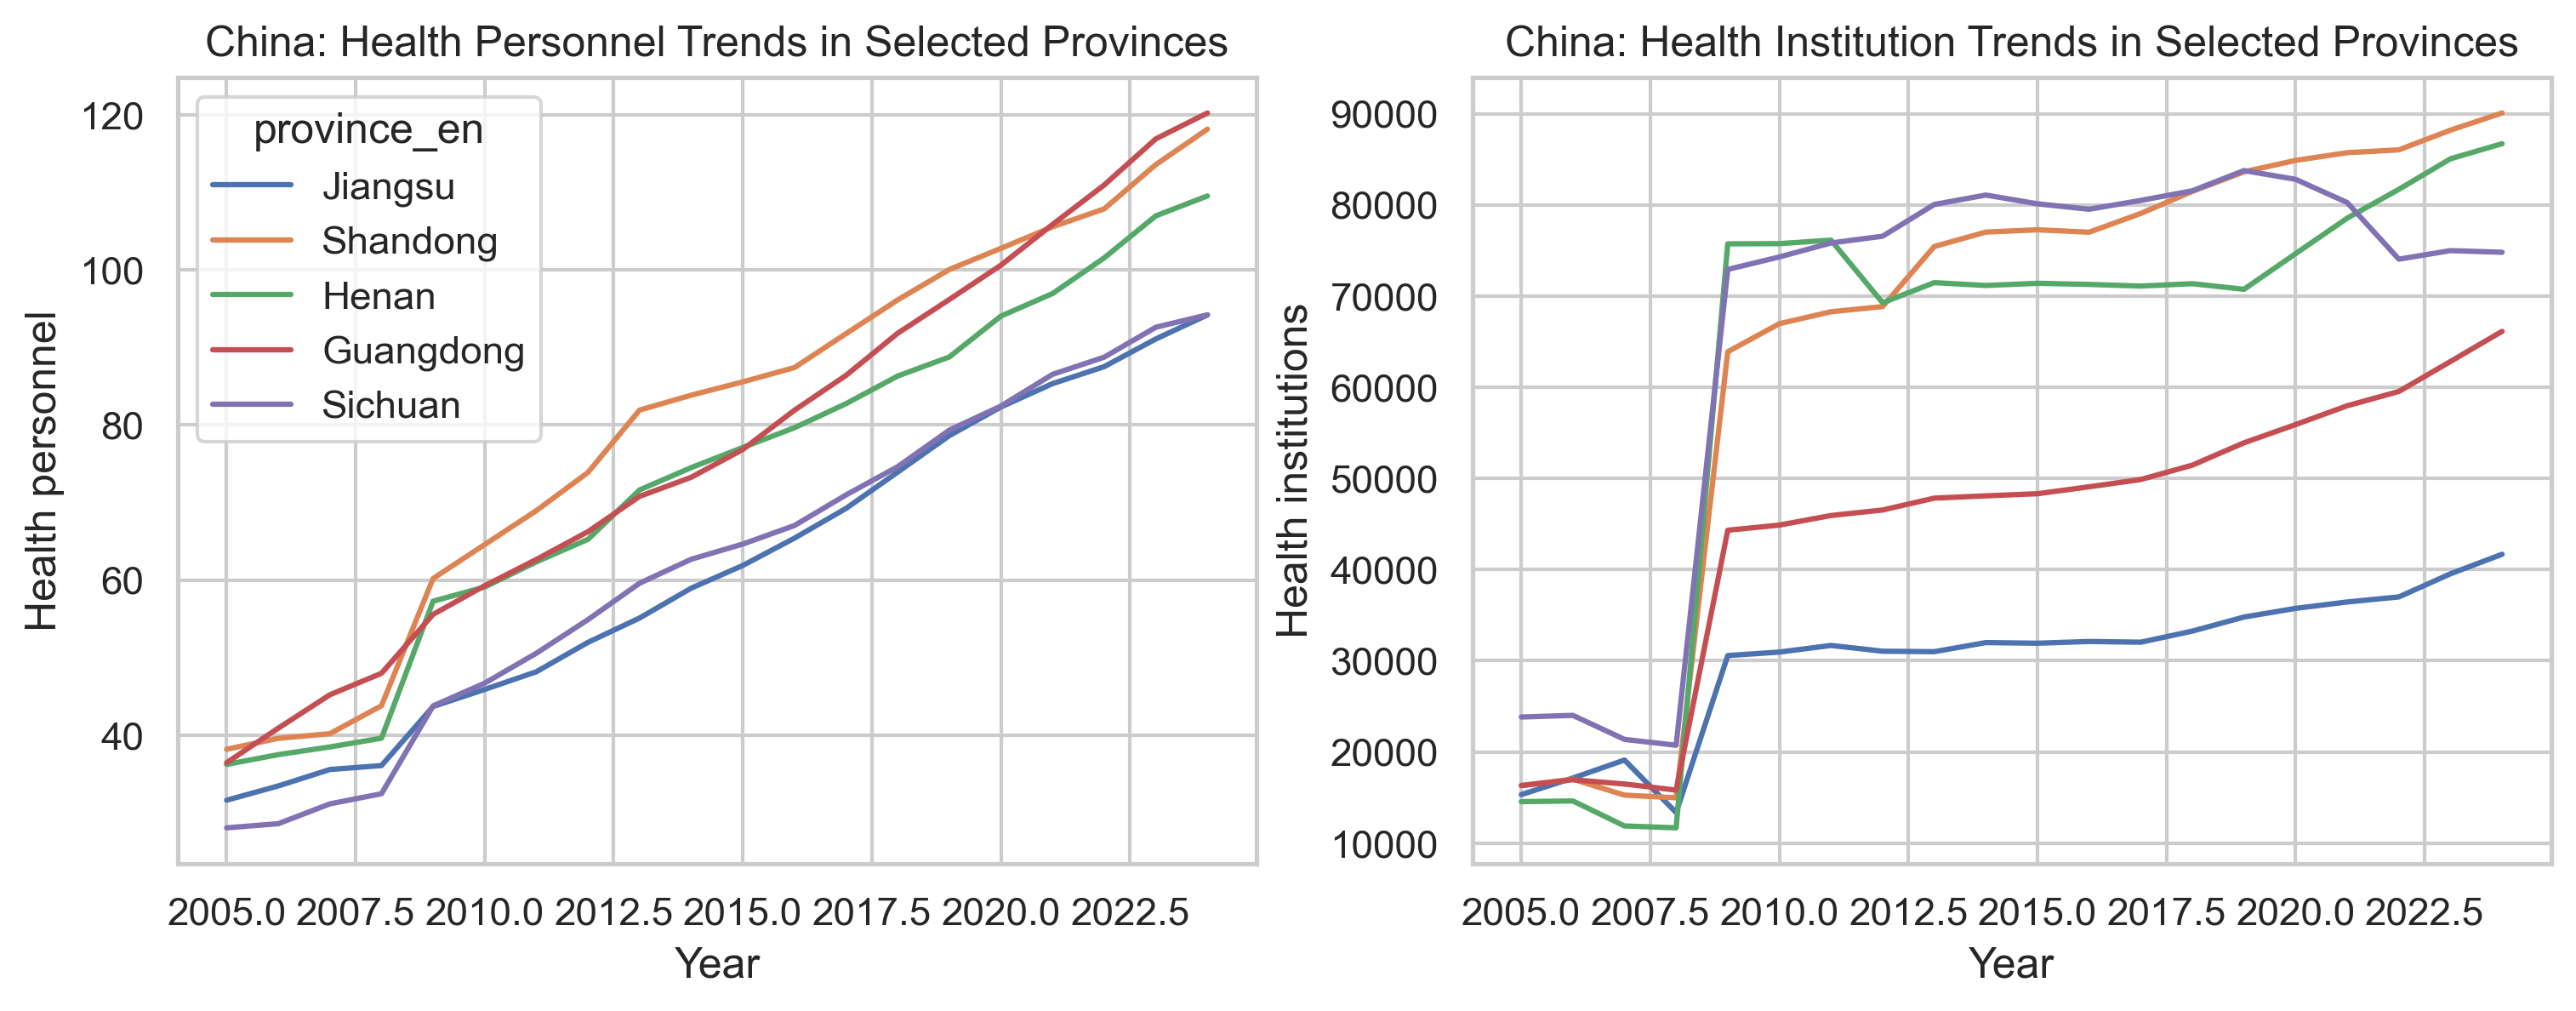
\includegraphics[width=0.9\textwidth]{figures/fig08_china_province_trends.png}
    \caption{中国重点省份卫生人员与机构数量趋势}
    \label{fig:china-trends}
\end{figure}

\section{AI 协作与可复现性}
本项目完整保留了与 AI 智能体的协作记录，包括任务理解、数据结构辨识、代码生成、调试与结果解释等环节。与最终交付一并提供的材料包括：
\begin{itemize}[leftmargin=1.5em]
    \item \texttt{ai\_agent/workflow.md}：协作流程说明；
    \item \texttt{ai\_agent/interaction\_logs/*.json}：对话日志样例；
    \item \texttt{api\_output/}：静态 API JSON 结果；
    \item \texttt{data/processed/*.parquet}：处理后的分析面板。
\end{itemize}

\section{结论与局限}
本研究基于 provided 数据完成了一个更贴近赛题数据结构的健康生态分析框架。核心结论有三点：
\begin{enumerate}[label=\arabic*)]
    \item 全球疾病谱已经显著转向非传染性疾病主导，但低寿命国家仍然表现出更高的传染性疾病占比；
    \item 高血压是 2023 年全球最重要的风险因素，但 AFRO 的首要矛盾仍集中于营养不良与基础公共卫生条件；
    \item 卫生资源缺口具有明显的地区集中性，且部分“低投入--高产出”国家提示了效率提升与经验复制的可能性。
\end{enumerate}

本项目的主要局限在于：赛题第二类数据提供的是归因死亡结果，而非严格的暴露率与 RR 参数，因此 Dimension 2 的主口径是“归因死亡贡献分析”而不是教科书意义上的 PAF 估计；同时，当前环境缺少本地 TeX 编译链，因此本次交付以完整 LaTeX 源文件为主，PDF 可在具备 XeLaTeX 的环境中直接编译。

\section*{参考文献}
\begin{enumerate}[leftmargin=1.5em]
    \item 2026 年（第 19 届）中国大学生计算机设计大赛大数据主题赛“健康数据洞察”赛题说明。
    \item World Bank. World Development Indicators.
    \item World Bank. Health Nutrition and Population Statistics.
\end{enumerate}

\appendix
\section{补充说明}
\begin{itemize}[leftmargin=1.5em]
    \item 主分析结果均可由 \texttt{python -m hdi.data.integrator} 与 \texttt{python -m hdi.analysis.competition} 复现。
    \item GHRI 未作为本次主线结果提交，但保留了元数据占位接口，以避免旧前端或旧 API 逻辑报错。
\end{itemize}

\end{document}
